% Activate the following line by filling in the right side. If for example the name of the root file is Main.tex, write
% "...root = Main.tex" if the chapter file is in the same directory, and "...root = ../Main.tex" if the chapter is in a subdirectory.
 
%!TEX root =  dissertation.tex

\chapter[Analysis]{Analysis}

\section{Usability result and analysis}

In evaluating HemeWeb's usability and capability to run and reproduce simulation, I conducted a usability evaluation via an online survey hosted by Google Form\footnote{\url{https://goo.gl/forms/toYsRwnGIGumMBUD2}}. Respondents are given 2 tasks to complete, which are to run a simulation and reproduce a past simulation. After the tasks, they are given statements to respond to. Based on the answers, I can make an analysis about HemeWeb's usability.


\subsection{Demography}


\vspace{0.5cm}

\noindent%
\begin{minipage}{\linewidth}% to keep image and caption on one page
\makebox[\linewidth]{
  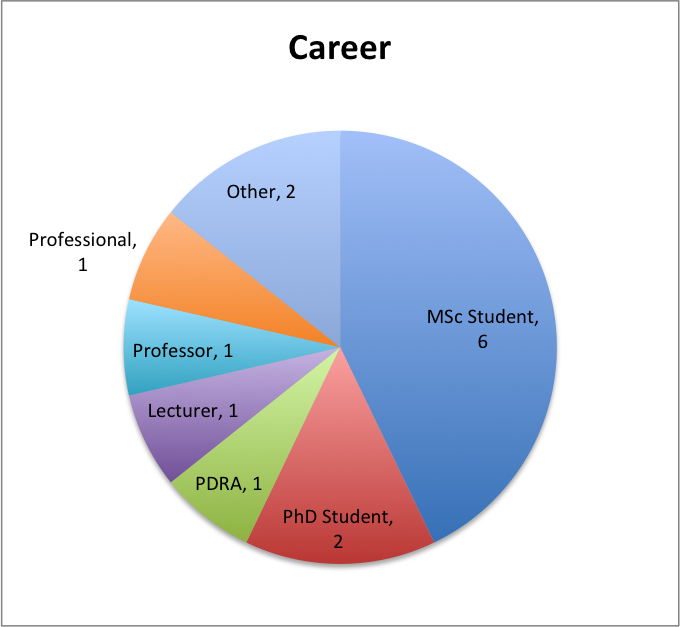
\includegraphics[keepaspectratio=true,scale=0.7]{../resources/evaluation/usability/career.png}
 }
\captionof{figure}{Career stage distribution} \label{fig:survey-career}%      only if needed  
\end{minipage}

\vspace{0.5cm}

\vspace{0.5cm}

\noindent%
\begin{minipage}{\linewidth}% to keep image and caption on one page
\makebox[\linewidth]{
  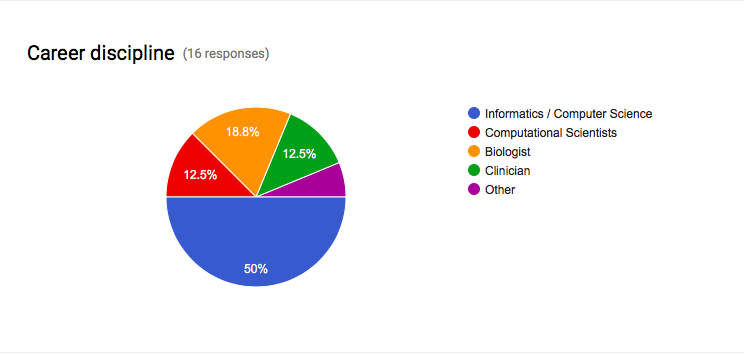
\includegraphics[keepaspectratio=true,scale=0.8]{../resources/evaluation/usability/discipline.png}
 }
\captionof{figure}{Career discipline} \label{fig:survey-discipline}%      only if needed  
\end{minipage}

\vspace{0.5cm}


The survey was filled by 16 respondents over the period of 10 days (3rd August 2016 - 12th August 2016)\footnote(See Appendix \ref{app:feedback}) \footnote{Raw and compiled responses can be found at \url{https://github.com/SeiryuZ/HemeWeb/tree/master/documents/resources/evaluation/usability} \label{footnote:response}}. From all the responses, one of the respondent was unable to run both of the tasks, citing errors preventing him to run the scenarios which we cannot reproduce. Another respondent also skip the second scenario without specifying reasons or contacting the author. Due to this problem, we have to remove these two responses from our analysis because it will not add meaningful information about the usability of the system when the scenarios are not run. In total, we got 14 valid responses out of the questionnaire period.

Figure \ref{fig:survey-career} and \ref{fig:survey-discipline} illustrates the distribution of career stage and discipline of our participants. Based on this distribution, we can further analyze the response we get on the survey questions based on their background. One meaningful comparison we can make is when we classify respondents based on their informatics-related discipline. 10 of our respondents are related to informatics background, while 4 of the respondents can be considered as domain experts which consists of Biologist, Clinician, and Biophysicist.


\vspace{0.5cm}

\noindent%
\begin{minipage}{\linewidth}% to keep image and caption on one page
\makebox[\linewidth]{
  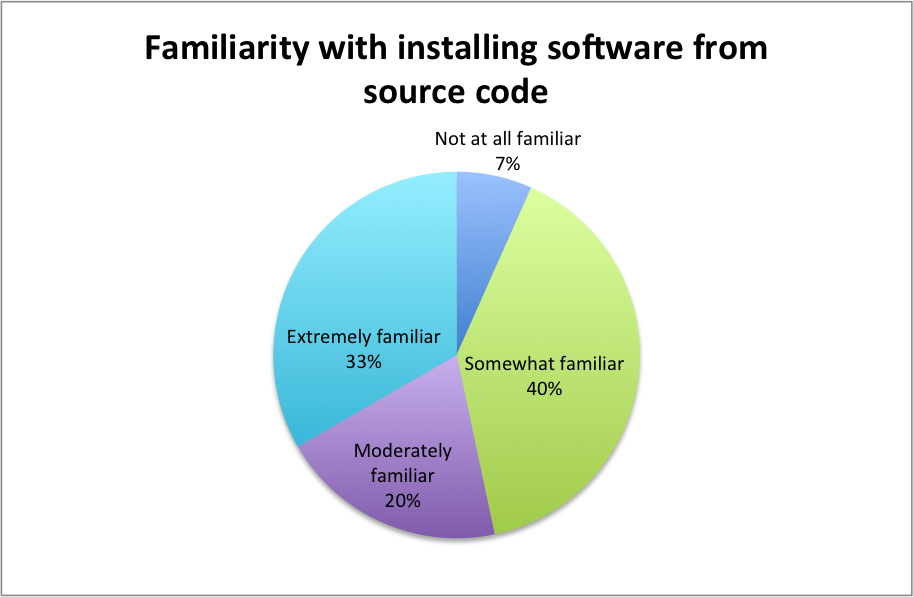
\includegraphics[keepaspectratio=true,scale=0.8]{../resources/evaluation/usability/source_code.png}
 }
\captionof{figure}{Familiarity with installing software from source code} \label{fig:survey-source}%      only if needed  
\end{minipage}

\vspace{0.5cm}

\noindent%
\begin{minipage}{\linewidth}% to keep image and caption on one page
\makebox[\linewidth]{
  
\includegraphics[keepaspectratio=true,scale=0.8]{../resources/evaluation/usability/browser.png}
 }
\captionof{figure}{Familiarity with web browser} \label{fig:survey-browser}%      only if needed  
\end{minipage}

\vspace{0.5cm}

\noindent%
\begin{minipage}{\linewidth}% to keep image and caption on one page
\makebox[\linewidth]{
  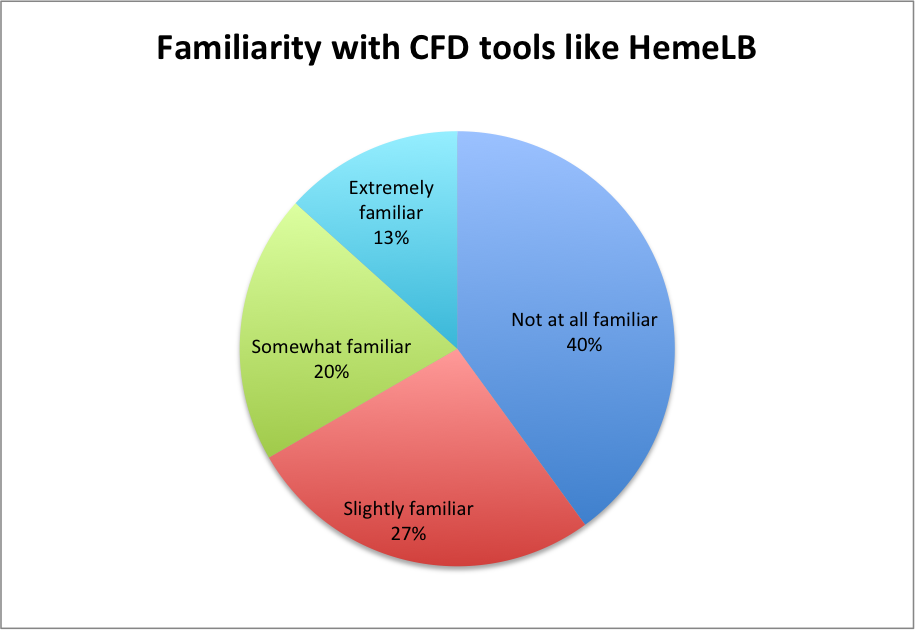
\includegraphics[keepaspectratio=true,scale=0.8]{../resources/evaluation/usability/hemelb.png}
 }
\captionof{figure}{Familiarity with CFD tools like HemeLB} \label{fig:survey-hemelb}%      only if needed  
\end{minipage}

\vspace{0.5cm}


We can also further classify analyze the respondents' response based on the familiarity with browsers, computational fluid dynamic tools, and installing software from source code. All of this are shown in Figure \ref{fig:survey-source}, \ref{fig:survey-browser}, and \ref{fig:survey-hemelb}.



\subsection{Scenario 1: Run a HemeLB simulation}

In this scenario, respondents are provided with two input files necessary for running a simulation. Respondents are asked to download the files beforehand and follow the instructions provided in the online questionnaire to run a HemeLB simulation using HemeWeb.  After running the simulation, Respondents are then asked to state agreement with three positive statements about HemeWeb that will measure their satisfaction with HemeWeb in running a HemeLB simulation scenario. 



\vspace{0.5cm}

\noindent%
\begin{minipage}{\linewidth}% to keep image and caption on one page
\makebox[\linewidth]{
  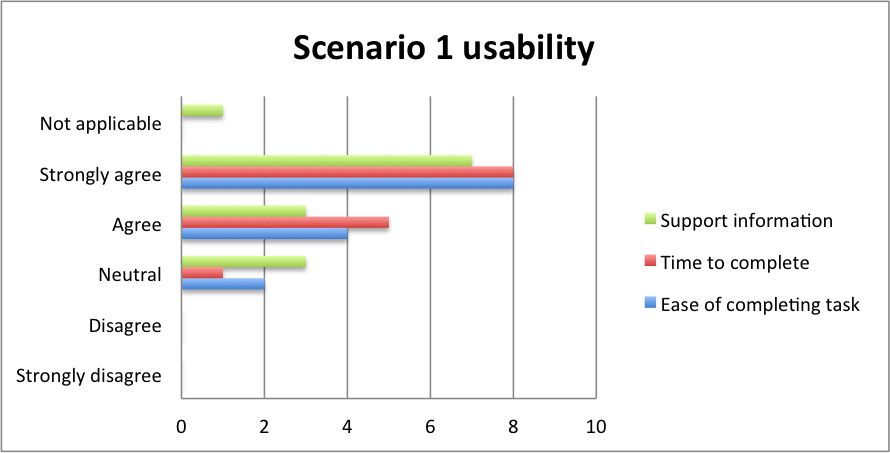
\includegraphics[keepaspectratio=true,scale=0.9]{../resources/evaluation/usability/scenario1_usability.png}
 }
\captionof{figure}{Scenario 1 usability} \label{fig:survey-s1-usability}%      only if needed  
\end{minipage}
\vspace{0.5cm}


Figure \ref{fig:survey-s1-usability} show the responses for the three positive statements about HemeWeb. From the 14 valid responses we get, all of them did not skip the instructions to run the simulation. From the responses, respondents tend to agree that they are satisfied with HemeWeb in running a HemeLB simulation. Respondents tend to equally agree on the three positive statements about the ease of completing a task, time to complete, and supporting information available to help complete the task. However, one respondent fills out "Not Applicable" towards the statement about HemeWeb giving them enough support information. 

In addition to the general sentiment of the respondents, we can also put a number value to the responses to further measure the satisfaction objectively. We can calculate the After Scenario Questionnaire(ASQ) score. To do this, we assign an integer value for each response; 1 for "Strongly disagree", 2 for "Disagree", 3 for "Neutral", 4 for "Agree", and 5 for "Strongly agree". With this value, we can take the mean of the response for each question as a single ASQ score for the respondent. If a respondent skips a question, we can take the average of the remaining responses as the score. With this mechanism, we can calculate the respondent's average ASQ score, which is 4.4 when rounded. This score falls between "Agree" and "Strongly agree", therefore, we can conclude that in general respondents are satisfied with HemeWeb with regards to running a HemeLB simulation.



%Our hypothesis is that users will generally find using web interface is usable and the data seemed to support that. It is much easier for user to complete a task when using point and click interface rather than requiring them to recall commands to do the tasks, especially when they are not familiar with the tools.
%
%
%Next, respondents are given a high overview of replicating the tasks done in HemeWeb but using command line interface. Respondents are not asked to run the scenario in their command line interface because we cannot make sure the necessary tools are installed on respondent's computer.

\vspace{0.5cm}

\noindent%
\begin{minipage}{\linewidth}% to keep image and caption on one page
\makebox[\linewidth]{
  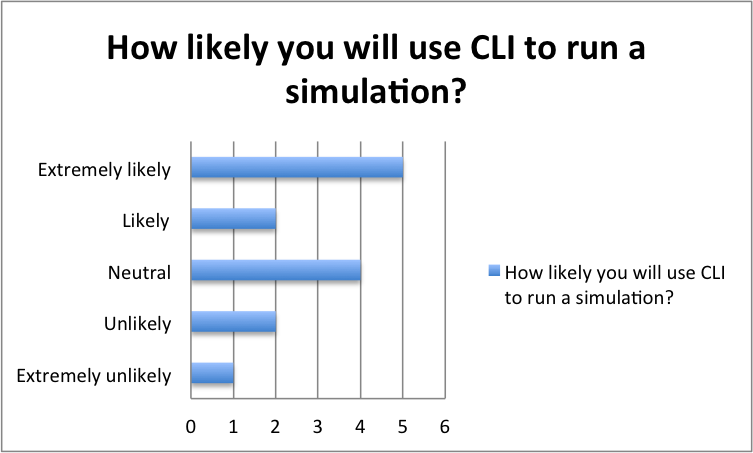
\includegraphics[keepaspectratio=true,scale=0.9]{../resources/evaluation/usability/scenario1_cli.png}
 }
\captionof{figure}{Scenario 1 command line preference} \label{fig:survey-s1-cli}%      only if needed  
\end{minipage}

\vspace{0.5cm}

\noindent%
\begin{minipage}{\linewidth}% to keep image and caption on one page
\makebox[\linewidth]{
  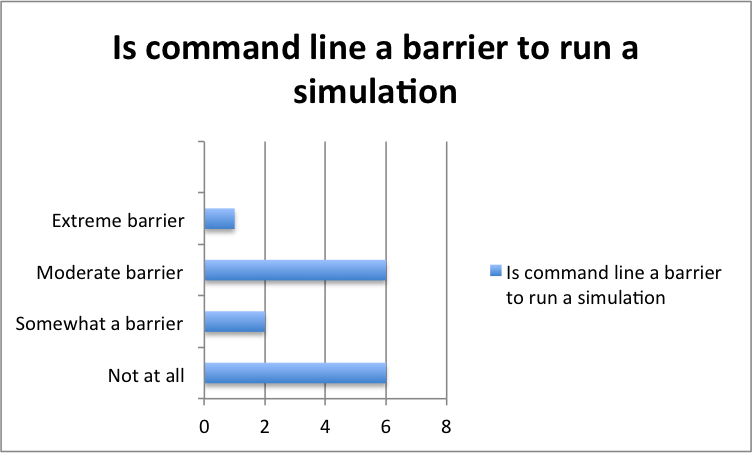
\includegraphics[keepaspectratio=true,scale=0.9]{../resources/evaluation/usability/scenario1_cli_barrier.png}
 }
\captionof{figure}{Scenario 1 barrier in using command line} \label{fig:survey-s1-cli-barrier}%      only if needed  
\end{minipage}

\vspace{0.5cm}

After the above sentiments about using HemeWeb to run a HemeLB simulation, respondents were asked about their sentiment about using Command Line Interface(CLI) to do the same activity. Figure \ref{fig:survey-s1-cli} and \ref{fig:survey-s1-cli-barrier} shows the respondent's responses. Respondents are generally open to the likelihood of them running a simulation using CLI. If we quantify the results like we did with the ASQ score, we get 3.6, which is between neutral and likely. 

The distribution of the responses also is quite spread out, that respondents fill out all possible responses with   the highest frequency being "Extremely Likely" with 5 responses. However, we have to keep it mind the general background of the respondents that may explain the highest frequency answer being "Extremely Likely", which is about familiarity with installing software with source code. To build software with source code, one will interact with the command line interface quite often. Thirteen of our respondents answered at least somewhat familiar with building software from source code, that can explain that our respondents are mostly quite competent in operating command line interface and would not shy away in using the command line interface. In addition to that, two out of three respondents has backgrounds in informatics and computational science. This could in effect explains why the respondents feel they are likely and extremely likely to do the same in CLI. 

However, not all respondents who are at least somewhat familiar with building software from source code skew towards to the likely side of using CLI. There are respondents that, while familiar with the interface, running a HemeLB simulation using CLI is unlikely to be done by them. These responses might be explained by respondents' sentiment in using command line interface. This is further supported by the response of CLI being a barrier for the respondents. While six of the respondents think it is not a barrier at all to use CLI, eight of the respondents answered at least it is somewhat a barrier. With five of the nine respondents, feel it is a moderate barrier, and one of the nine feel it as an Extreme barrier. From these results, we can safely say that using command line interface is a form of a barrier to run HemeLB for almost 60\% of the respondents, with this figure going up to 75\% when only the answers of the domain experts are considered.





\subsection{Scenario 2: Reproduce a past simulation}

In the second scenario, respondents are asked to reproduce past simulation with HemeWeb. They are given instructions in the online questionnaire to create a HemeLB simulation job from past simulation. They have to enter a URL that contains past simulation job and modifies the simulation parameters to avoid only replicating the past simulation without changes. After reproducing past simulation, respondents are then asked to state agreement with the same questions like they had in the first scenario. These questions will also measure their satisfaction with HemeLB in reproducing past simulation.


\vspace{0.5cm}

\noindent%
\begin{minipage}{\linewidth}% to keep image and caption on one page
\makebox[\linewidth]{
  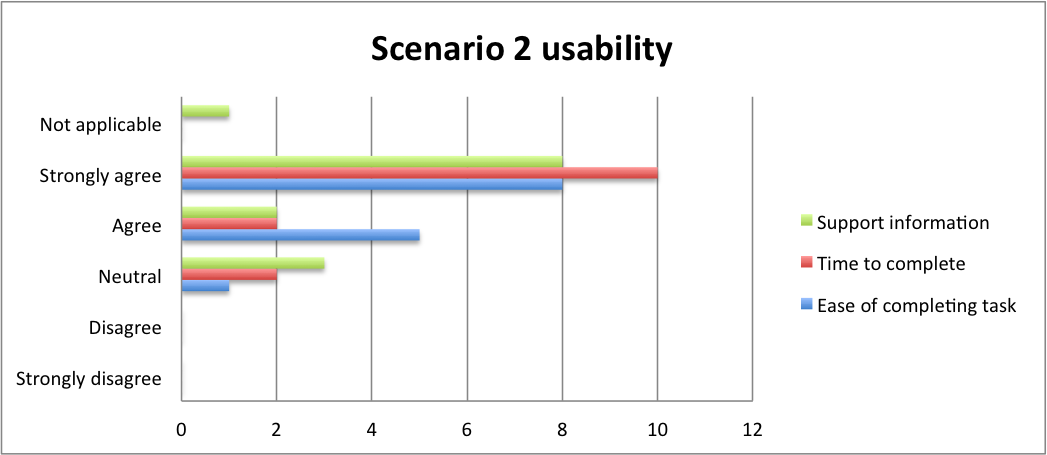
\includegraphics[keepaspectratio=true,scale=0.9]{../resources/evaluation/usability/scenario2_usability.png}
 }
\captionof{figure}{Scenario 2 usability} \label{fig:survey-s2-usability}%      only if needed  
\end{minipage}
\vspace{0.5cm}

Figure \ref{fig:survey-s2-usability} shows the general sentiment to the three statements that we provided. Generally, the response tends to skew towards agreeing that respondents are satisfied with HemeWeb with regards to reproducing past simulation. However, it has to be noted that 1 of the respondent skipped the instructions. This particular respondent did not give out any comments about encountering any problems, so we cannot deduce whether his skipping the instruction is due to usability problems or he just wants to skip it. Without further information, we cannot deduce why he skips the instructions and his response is one of the two taken out from the overall responses.

Also, similar to the first scenario, one respondent fills out "Not Applicable" to support information statement. In a nutshell, respondents tend to agree that HemeWeb is satisfying to use for the purpose of reproducing past simulation. If we convert the responses to a numerical value, we will get 4.5 of ASQ score. Which is in line with the sentiment that I described. The ASQ score falls between agreeing and strongly agree towards the positive statements we provided.


\vspace{0.5cm}

\noindent%
\begin{minipage}{\linewidth}% to keep image and caption on one page
\makebox[\linewidth]{
  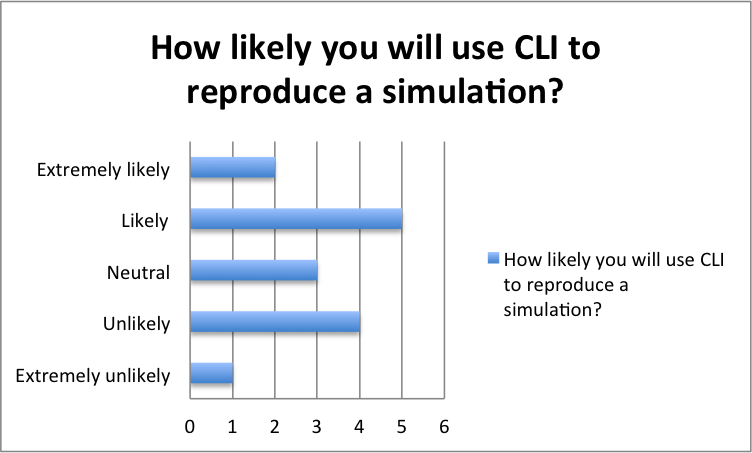
\includegraphics[keepaspectratio=true,scale=0.9]{../resources/evaluation/usability/scenario2_cli.png}
 }
\captionof{figure}{Scenario 2 command line preference} \label{fig:survey-s2-cli}%      only if needed  
\end{minipage}

\vspace{0.5cm}

\noindent%
\begin{minipage}{\linewidth}% to keep image and caption on one page
\makebox[\linewidth]{
  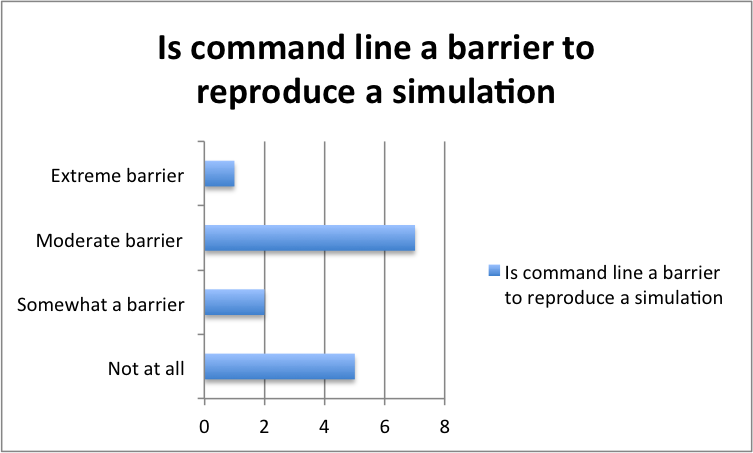
\includegraphics[keepaspectratio=true,scale=0.9]{../resources/evaluation/usability/scenario2_cli_barrier.png}
 }
\captionof{figure}{Scenario 2 barrier in using command line} \label{fig:survey-s2-cli-barrier}%      only if needed  
\end{minipage}

\vspace{0.5cm}

Respondents are then given high-level steps to reproduce past simulation using the command line interface.  Figure \ref{fig:survey-s2-cli} and \ref{fig:survey-s2-cli-barrier} shows the respondent's response. Similar to the first scenario, the respondents are generally open to the idea of operating command line interface to do their tasks. However, the scenario to reproduce past simulation provides a bit difference in the distribution of the answers. While in the first scenario the highest frequency of the answer is "Extremely likely", the highest frequency response in this scenario is "Likely". 

This change of the highest frequency might be because there are extra step which might complicate the scenario to reproduce past simulation. respondents are more hesitant to answer "Extremely likely". However, the general nuance of the answer is still the same, respondents are generally not afraid of using command line interface to do this task. If we convert the answers into a numerical form like we did before, we got 3.3, which is between neutral and likely. 

In addition, same observation as the first scenario can be made. While some respondents are likely to reproduce past simulations, there are those who are not likely to reproduce past simulations even with their background that have dealt with building software from source code. This can be explained by Figure \ref{fig:survey-s2-cli-barrier} where only five of the respondents did not feel that using CLI is a barrier at all. 2 of the respondents feel using CLI is somewhat a barrier, six feel it as a moderate barrier, and one feels it as an extreme barrier. This means that this nine respondents agree that CLI is a form of barrier to them, however small it is.


\subsection{Overall usability}


Here, I will discuss the overall usability of the system using the Post Study System Usability Questionnaire(PSSUQ) as the basis. This part of the questionnaire consists of 19 questions that can be divided into measuring three different component of the systems. These are system usefulness, information quality, and the interface quality. I will discuss each of them in details.

%%%%%%%%%%%%%%%%%%%%%%%%%%%%%%%%%%%
%  SYSTEM USEFULNESS 
%%%%%%%%%%%%%%%%%%%%%%%%%%%%%%%%%%%
\begin{center}
\captionof{table}{System usefulness}\label{table:overall-usability}
\scalebox{0.75}{

\begin{tabular}{|l|c|c|c|c|c|c|}
\hline
                                                                                                         & \multicolumn{1}{l|}{\begin{tabular}[c]{@{}l@{}}Strongly\\ disagree\end{tabular}} & \multicolumn{1}{l|}{Disagree} & \multicolumn{1}{l|}{Neutral} & \multicolumn{1}{l|}{Agree} & \multicolumn{1}{l|}{\begin{tabular}[c]{@{}l@{}}Strongly\\ agree\end{tabular}} & \multicolumn{1}{l|}{\begin{tabular}[c]{@{}l@{}}Not\\ applicable\end{tabular}} \\ \hline
\begin{tabular}[c]{@{}l@{}}Overall, I am satisfied with how easy it is\\ to use this system\end{tabular} & 0                                                                                & 0                             & 0                            & 7                          & 7                                                                             & 0                                                                             \\ \hline
It was simple to use this system                                                                         & 0                                                                                & 0                             & 0                            & 1                          & 13                                                                            & 0                                                                             \\ \hline
\begin{tabular}[c]{@{}l@{}}I can effectively complete my work\\ using this system\end{tabular}           & 1                                                                                & 1                             & 1                            & 3                          & 4                                                                             & 4                                                                             \\ \hline
\begin{tabular}[c]{@{}l@{}}I am able to complete my work quickly\\ using this system\end{tabular}        & 0                                                                                & 1                             & 2                            & 3                          & 6                                                                             & 2                                                                             \\ \hline
\begin{tabular}[c]{@{}l@{}}I am able to efficiently complete my work\\ using this system\end{tabular}    & 0                                                                                & 1                             & 2                            & 4                          & 5                                                                             & 2                                                                             \\ \hline
I feel comfortable using this system                                                                     & 1                                                                                & 0                             & 0                            & 3                          & 10                                                                            & 0                                                                             \\ \hline
It was easy to learn to use this system                                                                  & 0                                                                                & 0                             & 1                           & 0                          & 13                                                                            & 0                                                                             \\ \hline
\begin{tabular}[c]{@{}l@{}}I believe I became productive quickly\\ using this system\end{tabular}        & 0                                                                                & 0                             & 2                            & 3                          & 5                                                                             & 4                                                                             \\ \hline
\end{tabular}
}
\end{center}
\vspace{0.5cm}

Table \ref{table:overall-usability} shows the respondents sentiment towards positive statements about the system usefulness. Generally, we can see the distribution of respondents mostly agreeing with the statements presented. Ignoring the respondents that answered with "Not applicable", we can find the distribution is skewed to the agreeing side of the statements. There are respondents that disagree or even strongly disagree with some questions. However, the frequency is much lower compared towards the frequency of people agreeing to the statements. 

Converting  the response into a numerical value, we can get the score of 4.4 of system usefulness, which is quite high. However, there are still some improvements that can be made, and it is apparent in the feedbacks\footnote{See Appendix \ref{app:feedback} - Figure \ref{fig:survey-feedback}} of the system we got. For example, one respondent find the job configuration inflexible, another respondent find Firefox does not render the interface correctly. All of these can be addressed in the next iteration of HemeWeb development. In addition to these sentiments, there are respondents that respond to the statement by answering Not applicable. It is mostly on the framing of the simulation as a 'work'. Respondents might have no point of reference whether using the HemeLb via HemeWeb is quicker or efficiently because they are new to the system. This is apparent from their background that they don't  have familiarity with HemeLB.


%%%%%%%%%%%%%%%%%%%%%%%%%%%%%%%%%%%
%  INFO QUALITY
%%%%%%%%%%%%%%%%%%%%%%%%%%%%%%%%%%%

\begin{center}
\captionof{table}{Information quality}\label{table:overall-info-quality}
\scalebox{0.75}{
\begin{tabular}{|l|l|l|l|l|l|l|}
\hline
                                                                                                                                                                               & \begin{tabular}[c]{@{}l@{}}Strongly\\ disagree\end{tabular} & Disagree & Neutral & Agree & \begin{tabular}[c]{@{}l@{}}Strongly\\ agree\end{tabular} & \begin{tabular}[c]{@{}l@{}}Not\\ applicable\end{tabular} \\ \hline
\begin{tabular}[c]{@{}l@{}}The system gives error messages that\\  clearly tell me how to fix problems\end{tabular}                                                            & 0                                                           & 1        & 1       & 4     & 2                                                        & 6                                                        \\ \hline
\begin{tabular}[c]{@{}l@{}}Whenever I make a mistake using the system, \\ I recover easily and quickly\end{tabular}                                                            & 0                                                           & 0        & 4       & 1     & 3                                                        & 6                                                        \\ \hline
\begin{tabular}[c]{@{}l@{}}The information (such as online help, \\ on-screen messages, and other documentation)\\  provided with this system is clear\end{tabular}            & 0                                                           & 0        & 3       & 3     & 5                                                        & 3                                                        \\ \hline
It is easy to find the information I needed                                                                                                                                    & 0                                                           & 0        & 2       & 3     & 6                                                        & 3                                                        \\ \hline
\begin{tabular}[c]{@{}l@{}}The information (such as online help,\\  on-screen messages, and other documentation)\\  provided for the system is easy to understand\end{tabular} & 0                                                           & 0        & 2       & 5     & 6                                                        & 1                                                        \\ \hline
\begin{tabular}[c]{@{}l@{}}The information is effective in helping me\\  complete the tasks and scenarios\end{tabular}                                                         & 0                                                           & 1        & 3       & 2     & 7                                                        & 1                                                        \\ \hline
\begin{tabular}[c]{@{}l@{}}The organization of information on the \\ system screens is clear\end{tabular}                                                                      & 0                                                           & 0        & 2       & 8     & 4                                                        & 0                                                        \\ \hline
\end{tabular}

}
\end{center}
\vspace{0.5cm}

Table \ref{table:overall-info-quality} gives more insight on the respondents sentiment on HemeWeb's information quality. This includes information like error messages, documentation, the organization of this information, and etc. From seven positive statements that we presented. most respondents tend to agree that the information quality is good. The overall sentiment is more towards agreeing compared to disagreeing. If we convert the sentiment into a score, it will get 4.1 average score, Which falls under "Agree" and "Strongly agree" sentiment.  

However, there are more respondents answering "Not applicable" in this part of the questionnaire. This led to the remaining answer having more contribution towards the average sentiment because many of the answers are not counted. For example, there are 6 ignored responses on the first statement about error messages. This is likely because the scenario given to the respondents will not give out an error message if they are correct the first time.  In the end, however, respondents tend to agree that information quality of HemeWeb is good.




%%%%%%%%%%%%%%%%%%%%%%%%%%%%%%%%%%%
%  INTERFACE QUALITY
%%%%%%%%%%%%%%%%%%%%%%%%%%%%%%%%%%%
\begin{center}
\captionof{table}{Interface quality}\label{table:overall-interface-quality}
\scalebox{0.75}{
\begin{tabular}{|l|l|l|l|l|l|l|}
\hline
                                                                                                                  & \begin{tabular}[c]{@{}l@{}}Strongly\\ disagree\end{tabular} & Disagree & Neutral & Agree & \begin{tabular}[c]{@{}l@{}}Strongly\\ agree\end{tabular} & \begin{tabular}[c]{@{}l@{}}Not\\ applicable\end{tabular} \\ \hline
The interface of this system is pleasant                                                                          & 1                                                           & 0        & 1       & 7     & 5                                                        & 0                                                        \\ \hline
I like using the interface of this system                                                                         & 0                                                           & 1        & 1       & 8     & 4                                                        & 0                                                        \\ \hline
\begin{tabular}[c]{@{}l@{}}This system has all the functions and\\  capabilities I expect it to have\end{tabular} & 1                                                           & 1        & 1       & 4     & 4                                                        & 3                                                        \\ \hline
\end{tabular}
}
\end{center}
\vspace{0.5cm}


Table \ref{table:overall-interface-quality} shows the respondents sentiment with regards to HemeWeb's interface quality. In it, we see respondents strongly disagree and disagree with positive statements about the interface. While in general, most respondents tend to agree that the interface is good, some disagree. When we see this particular response, it seemed that the respondent had trouble with the interface not rendering correctly in firefox. This feedback means that the browser compatibility of HemeWeb should be improved. There are parts of the interface which are broken if it is viewed on firefox. There are other respondents who dislike the XML editor based on their feedbacks. However, all this are subjective in nature and further testing of the interface is needed.

However, if we convert the respondents answer to a numerical value, we got 4.0, which is "agree". It shows that while some respondents find the interface quality is not up to their standards, some find it good enough although a lot can be improved. Browser compatibility, web form choice, user experience, and etc should be improved on the next iteration of HemeWeb.



\begin{center}
\captionof{table}{Overall user satisfaction quality}\label{table:overall-satisfaction}
\scalebox{0.75}{
\begin{tabular}{|l|l|l|l|l|l|l|}
\hline
                                         & \begin{tabular}[c]{@{}l@{}}Strongly\\ disagree\end{tabular} & Disagree               & Neutral                & Agree                  & \begin{tabular}[c]{@{}l@{}}Strongly\\ agree\end{tabular} & \begin{tabular}[c]{@{}l@{}}Not\\ applicable\end{tabular} \\ \hline
Overall, I am satisfied with this system & \multicolumn{1}{c|}{0}                                      & \multicolumn{1}{c|}{0} & \multicolumn{1}{c|}{1} & \multicolumn{1}{c|}{7} & \multicolumn{1}{c|}{6}                                   & \multicolumn{1}{c|}{0}                                   \\ \hline
\end{tabular}
}
\end{center}
\vspace{0.5cm}

The last part of the question is the overall perceived satisfaction that the user has in using the system. The distribution of the response can be found in Table \ref{table:overall-satisfaction}. Most of the respondents gravitate towards agreeing and strongly agreeing that they are satisfied with the system. When we convert it into a numerical mean, it is 4.4, which is between "Agree" and "Strongly agree". To get the overall user satisfaction score of the study, we average the numerical score between the 19 questions and we got 4.2. This means that the respondents mostly agree that they are satisfied with how the system performs,  inform, and looks like.




\section{Performance result and analysis}

In this section, I will discuss the performance benchmark of HemeLB simulation done in three infrastructure, ARCHER supercomputer, INDY2 HPC cluster, and AWS EC2. Understanding the difference in performance is essential for HemeWeb project to justify the flexibility that cloud vendors provide.

In this benchmark, we are going to rely on the report file that HemeLB produced. It is produced after each simulation is done and contains performance metric of each simulation like how many seconds are spent on communication, initializations, reading input files, and most importantly total simulation time. We are going to take a look at the total simulation time because it is the metric that captures the difference in the infrastructure better. We ran the exact same simulation scenario on all three infrastructure . On each infrastructure, the simulations were done with an increasing number of compute node to measure the scalability of HemeLB.  From the produced output, then we can measure the performance difference between architecture.





\begin{center}

\captionof{table}{HemeLB performance on INDY2 vs ARCHER vs AWS EC2. Results for ARCHER and INDY2 run provided by Dr. Rupert Nash}\label{table:perf}

\begin{tabular}{|c|c|c|c|c|c|c|}
\hline
\multirow{2}{*}{\# Compute node(s)} & \multicolumn{2}{c|}{INDY2} & \multicolumn{2}{c|}{ARCHER} & \multicolumn{2}{c|}{AWS-EC2} \\ \cline{2-7} 
                                  & Core       & Time / s      & Core       & Time / s       & Core        & Time / s       \\ \hline
1                                 & 36         & 24.7          & 24         & 33.6           & 18          & 35.3           \\
2                                 & 72         & 12.7          & 48         & 22.1           & 36          & 24.6           \\
4                                 & 144        & 7.08          & 96         & 13.4           & 72          & 16.8           \\
8                                 & 288        & 3.44          & 192        & 9.81           & 144         & 11.5           \\
16                                 & 576        & 1.81          & 384        & 9.94           & 288         & 10.3           \\
32                                 & 1152       & 1.58          & 768        & 9.64           & N/A         & N/A            \\ \hline
\end{tabular}

\end{center}



\vspace{0.5cm}


\noindent%
\begin{minipage}{\linewidth}% to keep image and caption on one page
\makebox[\linewidth]{
  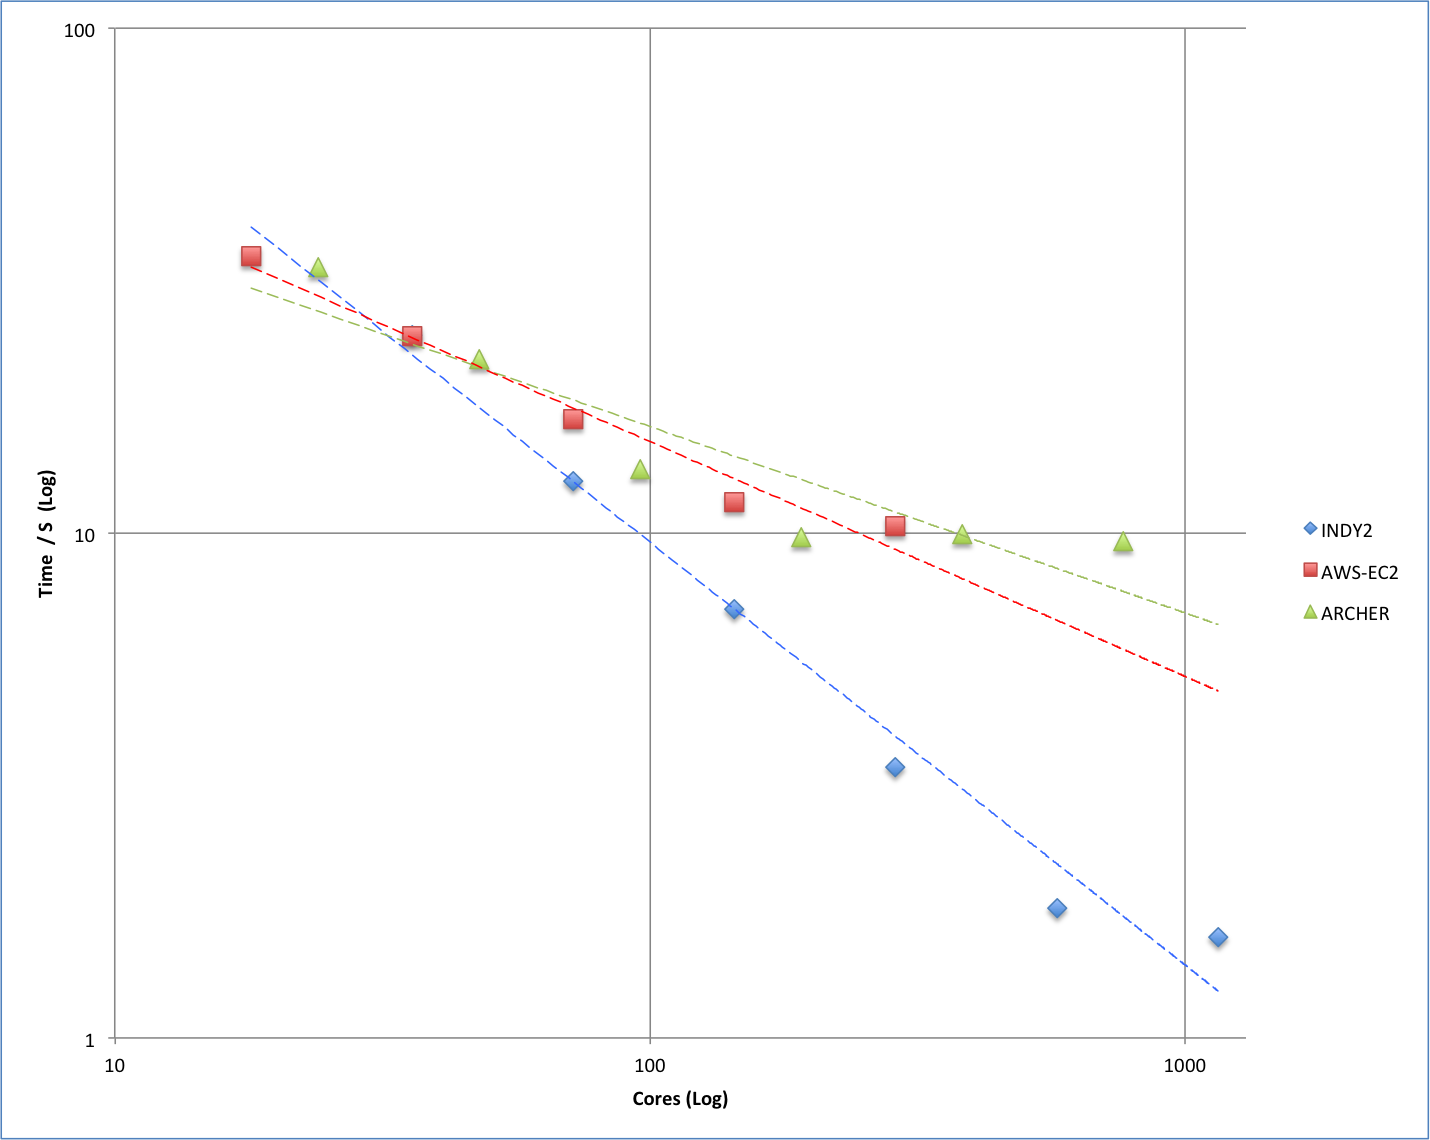
\includegraphics[keepaspectratio=true,scale=0.70]{../resources/evaluation/performance/overview.png}
 }
\captionof{figure}{HemeLB performance comparison. Results for ARCHER and INDY2 run provided by Dr. Rupert Nash} \label{fig:hemelb-perf-overview}%      only if needed  
\end{minipage}

\vspace{0.5cm}


Table \ref{table:perf} shows the performance comparison between HemeLB total simulation time between AWS-EC2, INDY2, and ARCHER. It shows that AWS-EC2 perform relatively well in lower amount of cores used. At 36 cores, AWS-EC2 perform even slightly better compared to INDY2. It has to be noted that AWS-EC2 has lower core count in a single compute node compared to ARCHER that makes direct comparison impossible. However, we can see from the simulation time that AWS-EC2 perform relatively well compared to ARCHER's performance because it has small difference of the performance despite the lower core count. 


Another observation that can be made from the performance information, is that AWS-EC2 performance experienced a bigger performance degradation on increased core counts compared to the other two infrastructures.  This shows that while the raw performance of the compute cores are very respectable, the parallel scalability of AWS EC2 is not as good as the other two infrastructures.

% This shows that AWS-EC2 performance is much slower compared to the dedicated infrastructure likes INDY2 and ARCHER. AWS-EC2 is slower 3-25\% compared to ARCHER, and 42-469\% compared to INDY2 on various compute node size. However, it has to be noted  that on each infrastructure, one compute node have different core count. This could affect the performance difference we got from this result.

Figure \ref{fig:hemelb-perf-overview} also shows the difference in performance between the three infrastructure. INDY2 performed much faster than the other infrastructures. In addition, its performance also scales almost linearly up to 576 cores and had a performance degradation on 1152 cores. This closely follows the performance analysis by Groen et al. \citep{groen2013analysing}. 

Next, ARCHER perform better than AWS-EC2. While it is still slower than INDY2, ARCHER provide more performance per compute nodes when we compare it to AWS-EC2. However, on 192 cores up to 768 cores, the performance became stagnant. It didn't achieve a better improvement as we scale. The performance difference between INDY2 and ARCHER can be explained by the different load on each system at the time of benchmark. INDY2 is on the early-access testing phase where at the time of execution, Dr. Rupert Nash was the only person using the infrastructure. On the other hand, when Dr. Rupert Nash executed HemeLB on ARCHER, the utilization was very high, which means that the HemeLB job potentially has to share network interconnectivity with other jobs.

Finally, AWS-EC2 perform slower on each compute nodes count we tested. The performance improved on increased the core count. However, this improvement is not nearly linear as modeled by Groen et al. \citep{groen2013analysing}. This result could have many causes, but generally still in line with the benchmark that Mehrotra et al. did on NASA's HPC application \citep{mehrotra2012performance}. The performance degradation comes from the network and the virtualization overhead that this cloud platform has. In addition, we do not have control over how the compute node are arranged on the cloud platform. We could have nodes with varying degree of interconnectivity on each simulation. A simulation might have started compute nodes near each other in the Amazon's data center, the next simulation might start compute nodes which need longer network interconnectivity. 

\begin{center}

\captionof{table}{HemeLB parallel efficiency table of INDY2 vs ARCHER vs AWS EC2. ARCHER and INDY2 result is based on the data provided by Dr. Rupert Nash}\label{table:eff}

\scalebox{0.75}{
\begin{tabular}{|c|c|c|c|c|c|c|c|c|}
\hline
\multicolumn{3}{|c|}{INDY2}      & \multicolumn{3}{c|}{ARCHER}      & \multicolumn{3}{c|}{AWS-EC2}     \\ \hline
Core & Speedup     & Efficiency  & Core & Speedup     & Efficiency  & Core & Speedup     & Efficiency  \\ \hline
36   & 1           & 1           & 24   & 1           & 1           & 18   & 1           & 1           \\
72   & 1.94488189  & 0.972440945 & 48   & 1.520361991 & 0.760180995 & 36   & 1.43495935  & 0.717479675 \\
144  & 3.488700565 & 0.872175141 & 96   & 2.507462687 & 0.626865672 & 72   & 2.101190476 & 0.525297619 \\
288  & 7.180232558 & 0.89752907  & 192  & 3.425076453 & 0.428134557 & 144  & 3.069565217 & 0.383695652 \\
576  & 13.64640884 & 0.852900552 & 384  & 3.38028169  & 0.211267606 & 288  & 3.427184466 & 0.214199029 \\
1152 & 15.63291139 & 0.488528481 & 768  & 3.485477178 & 0.108921162 & N/A  & N/A         & N/A         \\ \hline
\end{tabular}
}

\end{center}

\vspace{0.5cm}


\noindent%
\begin{minipage}{\linewidth}% to keep image and caption on one page
\makebox[\linewidth]{
  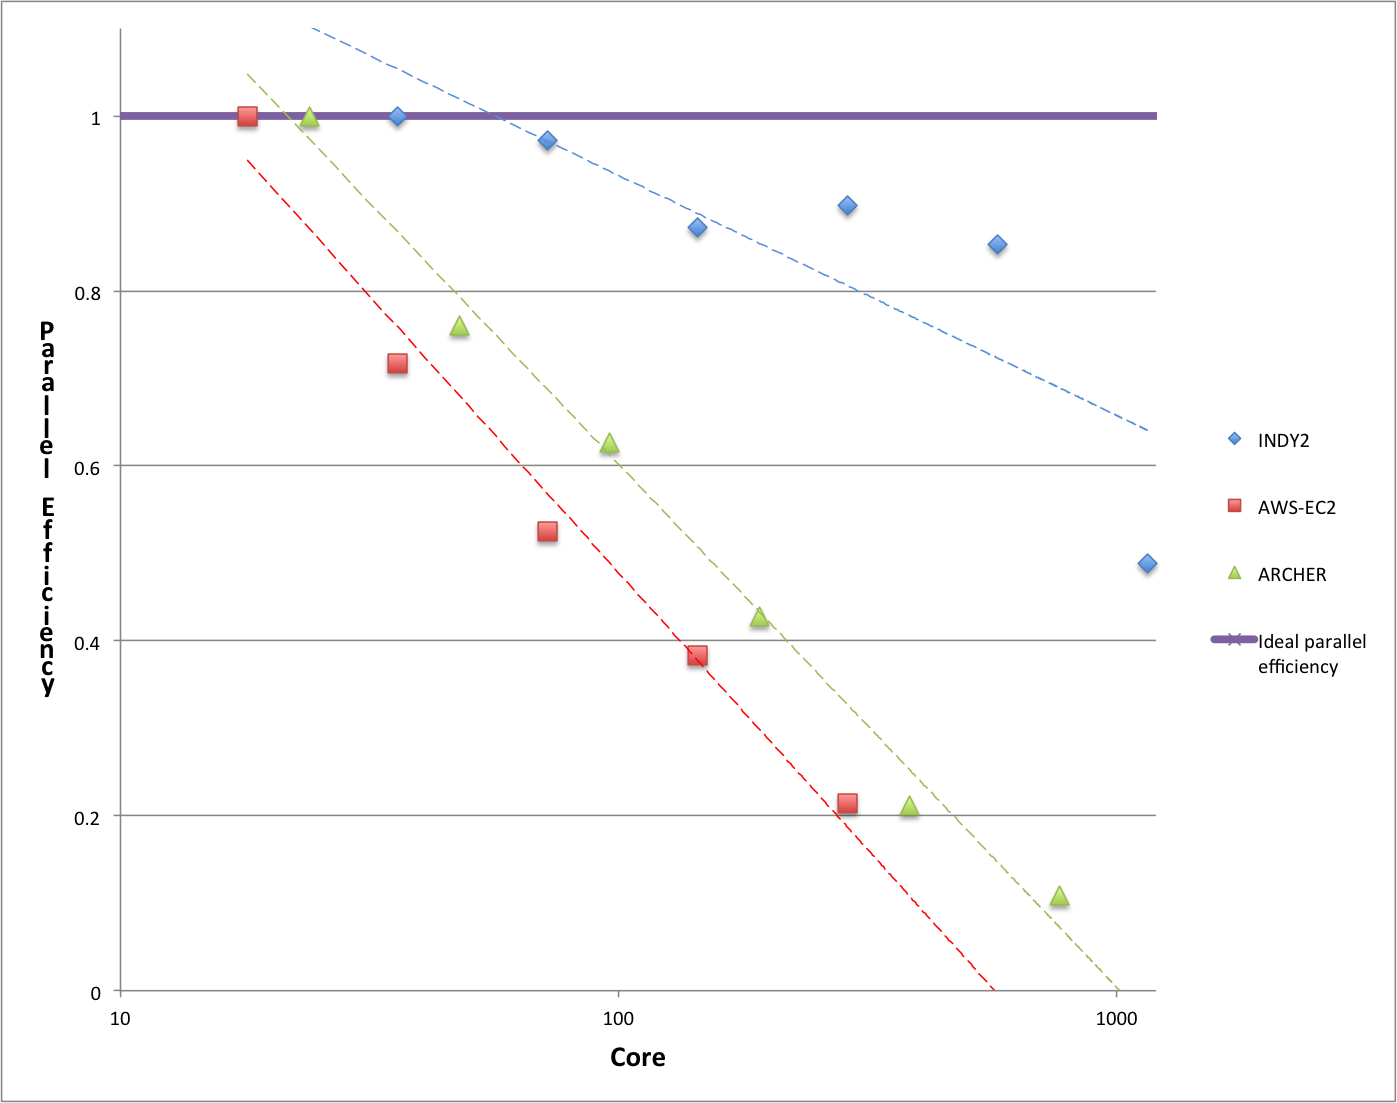
\includegraphics[keepaspectratio=true,scale=0.70]{../resources/evaluation/performance/efficiency.png}
 }
\captionof{figure}{HemeLB parallel efficiency plot. ARCHER and INDY2 result is based on the data provided by Dr. Rupert Nash} \label{fig:hemelb-eff-plot}%      only if needed  
\end{minipage}

\vspace{0.5cm}


From the raw performance information above, we can calculate the parallel scalability of HemeLB on all three infrastructure. Table \ref{table:eff} and Figure \ref{fig:hemelb-eff-plot} shows the difference of the parallel scalability on the three infrastructures with the basis of the smallest number of core used on each infrastructure. INDY2 has the best parallel scalability that it has the efficiency nearest to the ideal parallel scalability. However, the last data point produces a much slower speedup compared to other points that reduce its efficiency at 1,152 cores. 

ARCHER also perform better than AWS-EC2 in this evaluation. However, the parallel efficiency is still far below the level of INDY2 because of the utilization of the system. AWS-EC2 has the lowest parallel scalability as expected. This shows that running HemeLB on Amazon's infrastructure might not scale as well as using dedicated HPC infrastructure. However, on lower compute node count, AWS-EC2 provide a comparable parallel scalability (5\% difference) and performance compared to ARCHER under very high utilization. 


From the observations above, we can conclude  that that AWS-EC2 perform comparably to dedicated HPC infrastructure, especially on lower core count. However AWS-EC2 infrastructure does not scale as well as the dedicated HPC infrastructure. Based on this finding, we can further conclude that a small problem size that can be run on lower core count is an ideal use-case for HemeWeb because it will run with comparable performance with dedicated HPC infrastructure with the flexibility of cloud vendors.



\subsection{Simulation cost analysis}

In addition to performance analysis, we can further analyze the notional cost of a simulation job. For this, we need to come up with the way to calculate the simulation cost. This can be done by multiplying simulation time with cost per unit of time on that infrastructure.

\begin{displaymath}
 Simulation\ cost\ =\ simulation\ time\ X\ cost\ per\ unit\ of\ time\ x\ number\ of\ nodes
\end{displaymath}



In running the simulation for the benchmark, we used "c4.8xlarge" Linux instances on EU Ireland region which at the time of writing costs GBP 1.51\footnote{USD 1.96 converted to GBP on https://\url{www.oanda.com/currency/converter/} at 13th August 2016} per hour\footnote{\url{https://aws.amazon.com/ec2/pricing/}}. Phase 2 XC30 ARCHER supercomputer give access to screened projects by compute hour unit which has the price of GBP 0.20 per compute node for research councils which are partnered and GBP 0.48 per compute node for non-partnered research council\footnote{Calculated on \url{http://archer.ac.uk/access/au-calculator/}}. INDY2, however, have no public pricing released by the EPCC yet and cannot be included in this analysis. 


Calculating simulation time can be done by taking the performance of compute nodes on each infrastructure divided by the base time. The base time will be chosen from the fastest performance of the smallest compute node count on each infrastructure. In this evaluation, we ignore INDY2 because of missing pricing, so the base time is ARCHER with one compute node that runs for 33.6s. This will make sure that the simulation time across infrastructure shrinks relative to the performance of that time. With this information, we can finally calculate the simulation cost of using various compute nodes on each infrastructure.

\begin{displaymath}
 Simulation\ time\ ratio=\ simulation\ time\ /\ base\ time
\end{displaymath}

\begin{center}
\captionof{table}{HemeLB simulation cost on AWS-EC2 vs ARCHER. ARCHER and INDY2 result is based on the data provided by Dr. Rupert Nash}\label{table:cost}
\scalebox{0.75}{
\begin{tabular}{|c|c|c|c|c|c|}
\hline
Compute node & \begin{tabular}[c]{@{}c@{}}ARCHER time \\ difference ratio\end{tabular} & \begin{tabular}[c]{@{}c@{}}ARCHER-partner \\ simulation cost\end{tabular} & \begin{tabular}[c]{@{}c@{}}ARCHER-nonpartner\\ simulation cost\end{tabular} & \begin{tabular}[c]{@{}c@{}}AWS-EC2 time\\ difference ratio\end{tabular} & \begin{tabular}[c]{@{}c@{}}AWS-EC2\\ simulation cost\end{tabular} \\ \hline
1            & 1                                                                       & 0.2                                                                       & 0.48                                                                        & 1.05                                                                       & 1.59                                                              \\
2            & 0.66                                                             & 0.26                                                               & 0.63                                                                 & 0.73                                                             & 2.2                                                       \\
4            & 0.40                                                             & 0.32                                                               & 0.77                                                                 & 0.5                                                              & 3.02                                                       \\
8            & 0.30                                                             & 0.47                                                               & 1.12                                                                 & 0.34                                                             & 4.13                                                       \\
16           & 0.30                                                             & 0.95                                                               & 2.27                                                                       & 0.31                                                             & 7.41                                                       \\
32           & 0.29                                                             & 1.84                                                               & 4.41                                                                 & N/A                                                                     & N/A                                                               \\ \hline
\end{tabular}
}

\end{center}

\vspace{0.5cm}


\noindent%
\begin{minipage}{\linewidth}% to keep image and caption on one page
\makebox[\linewidth]{
  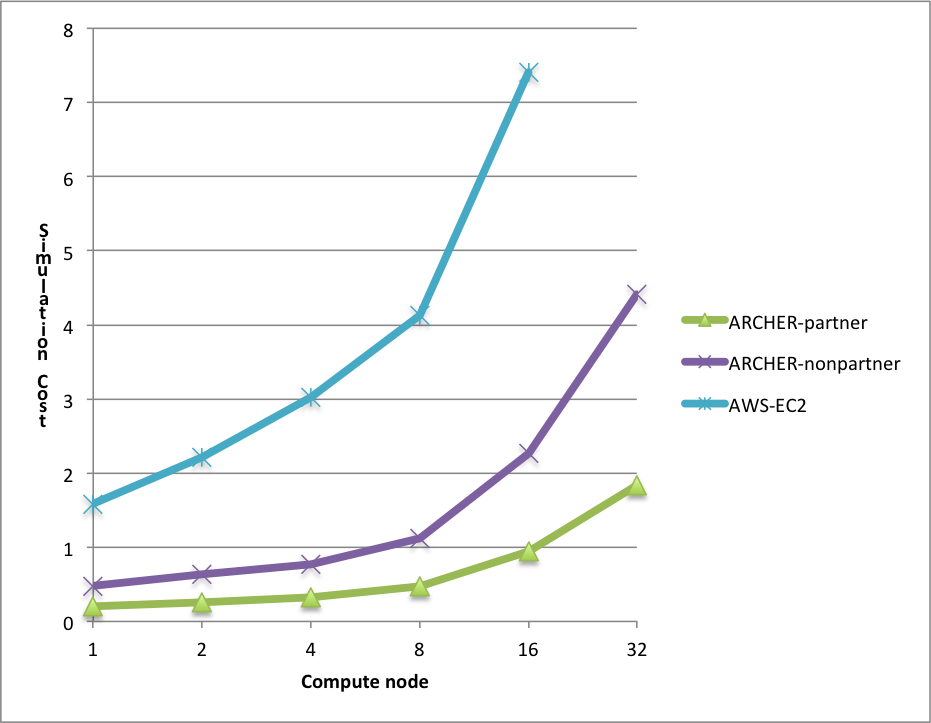
\includegraphics[keepaspectratio=true,scale=0.90]{../resources/evaluation/performance/cost.png}
 }
\captionof{figure}{HemeLB  simulation cost difference. ARCHER and INDY2 result is based on the data provided by Dr. Rupert Nash} \label{fig:hemelb-cost-plot}%      only if needed  
\end{minipage}

\vspace{0.5cm}

Table \ref{table:cost} shows the breakdown of simulation cost between AWS-EC2 with ARCHER with partner institutions and non-partner. From the calculation, AWS-EC2 is 680\% up to 850\% more costly compared to ARCHER with partner pricing. When we compare to the price of a non-research partner, we get 230\% to 290\% more cost to run a simulation. 


This result is as expected because, with slower performance, we are going to use compute nodes for longer. Longer usage means more cost to be paid by the users. In addition, cloud platform on AWS-EC2 rent out their services with a premium that allows a certain flexibility that dedicated HPC infrastructure like ARCHER cannot afford. This flexibility like the amount of time needed to first start running a simulation or running an exploratory experiments.

While being slower in running simulation, cloud vendors like Amazon web service allow domain experts to run simulation on-demand. On the contrary,  running a simulation,  even a small exploratory one, on dedicated HPC infrastructure like ARCHER, require users to apply for a spot, write a proposal, and wait for the next application decision. This is the time of doing simulation that cannot be measured by this evaluation and should be used as one of the basis of using HemeWeb on cloud vendors compared to dedicated HPC infrastructure.

This result means that if you are an existing scientists with access to HPC infrastructure like ARCHER, using HemeWeb might not be the best way to run your HemeLB simulation because of the costs. However, if you are a scientists with no access to HPC infrastructure like ARCHER or INDY2 and does not have a constant demand for compute hour for your simulation, HemeWeb may worth the cost compared to applying for a spot on these HPC infrastructures. In addition, the on-demand nature of HemeWeb fits perfectly with exploratory studies type of job which usually needs a one-off job with relatively small problem size. With HemeWeb, users can start running the simulation on-demand.





\section {Limitation of the evaluations}

\subsection{Usability evaluation}

When observing the evaluation, one might argue that 5 point scale used in the questionnaire is not enough as pointed out by Kraig Finstad \cite{finstad2010response}. In his research, he argued that 5 point scale for a questionnaire allows more room for respondents to interpolate their response. He compared the same version of usability study but with five-point and seven-point scale and found out that 3\% of the respondents answer to five point scale actually are interpolation, while the seven point scale have no interpolation. He concluded that administering usability study using seven point scale will achieve greater accuracy. However, I decided to use the five point scale of the questionnaire because of the limitation of google survey platform. 

\noindent%
\begin{minipage}{\linewidth}% to keep image and caption on one page
\makebox[\linewidth]{
  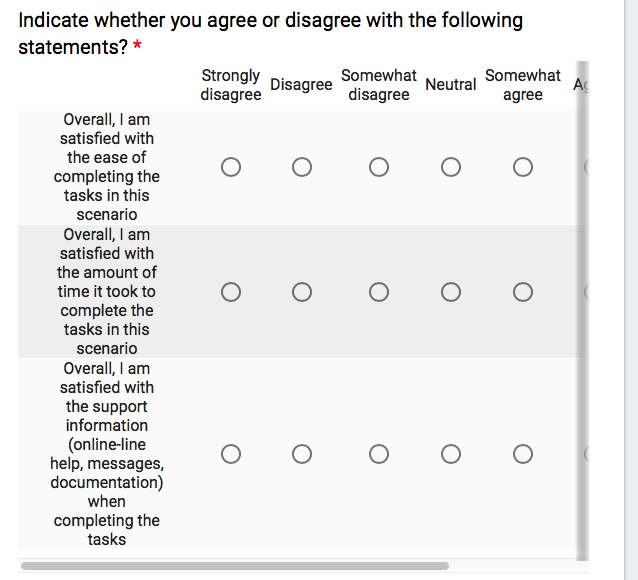
\includegraphics[keepaspectratio=true,scale=0.35]{../resources/images/google-limitation.png}
 }
\captionof{figure}{Google form hiding some options on 7 point scale} \label{fig:google-limit}%      only if needed  
\end{minipage}


\vspace{0.5cm}
\noindent%
\begin{minipage}{\linewidth}% to keep image and caption on one page
\makebox[\linewidth]{
  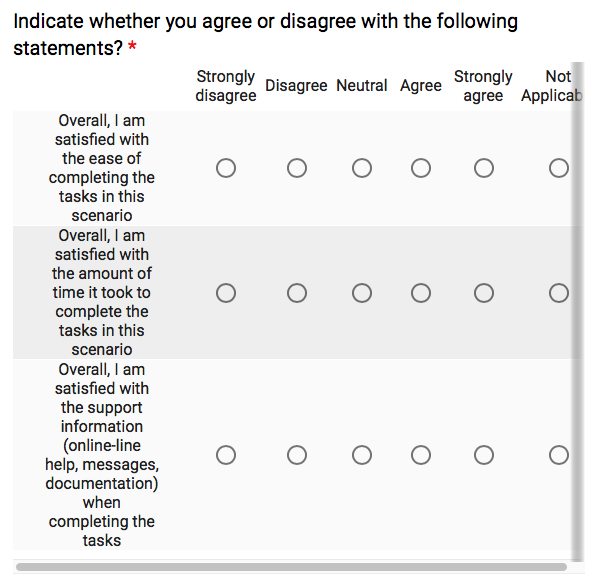
\includegraphics[keepaspectratio=true,scale=0.35]{../resources/images/google-limitation2.png}
 }
\captionof{figure}{Google form render 5 point scale rating better} \label{fig:google-limit2}%      only if needed  
\end{minipage}

\vspace{0.5cm}


Figure \ref{fig:google-limit} show the limitation of the platform. The response options are not rendered in complete, as in some are hidden in a scrolling element of the page. This leads to respondents have to scroll left and right to see the options and answers. I find this is a detriment to the respondents to do more work in answering the question so I decided to use 5 point scale to make sure everything is rendered better like shown in Figure \ref{fig:google-limit2}.


Another limitation of the study is the way the study compare the experience of doing the scenarios in the questionnaire between using web browser and using command line.  When measuring the usability of HemeWeb, respondents are asked to do the task in the web browser, compared to the task in command line where it is just described in an overview. This decision is made because we cannot make sure the respondents have the necessary tools to run or reproduce a simulation in their computers.  In addition, in order to run the scenario in command line interface, respondents have to install tools on their computer which are timely and prone to errors. I believe this will affect their sentiment in answering the survey questionnaire and decided against it.


\subsection{Performance evaluation}

On running the HemeLB simulation on the three systems compared, we cannot fully isolate the infrastructure from various system loads the infrastructure is handling. The performance might be affected by other jobs running in the system, which is apparent in the case of ARCHER supercomputer where many jobs are executing at the same moment. The same case with INDY2. The performance benchmark might be not as accurate as a completely isolated environment, however, it paints a pretty good picture of performance you get when using cloud vendors compared to the dedicated infrastructure. 

Also, another limitation on the performance evaluation is that we cannot get more than 20 instances of c4.8xlarge instances on AWS. This causes the evaluation for AWS-EC2 cannot be done for the 6 compute nodes to compare it directly with INDY2 and ARCHER. Another limitation is that each infrastructure has different core counts in their compute nodes. ARCHER has 24, INDY2 has 36, and AWS-EC2 has 18. Ideally, we want exact core count so we can make a direct comparison between each infrastructure, but this is not the case. However, it could help in painting the general trend of the scaling capabilities and performance measure based on the compute node count. 
